% ============================================================================
% SEC02.TEX - Section 7.2: Membuat Animasi Ledakan
% ============================================================================

\section{Membuat Animasi Ledakan}

Jika Anda tidak memiliki sprite sheet ledakan, Anda bisa membuatnya sederhana dengan mengubah Scale dan Transparency (Fade Out) dari sprite lingkaran.

\begin{enumerate}
    \item Buat GameObject Sprite baru (Circle), beri nama \texttt{ExplosionVFX}.
    \item Buka window \textbf{Animation} (\texttt{Window > Animation > Animation}).
    \item Klik tombol \textbf{Create} untuk membuat klip animasi baru. Beri nama \texttt{Explosion.anim}.
    \item Klik tombol \textbf{Record} (lingkaran merah).
    \item \textbf{0:00}: Biarkan Scale (1,1,1). Alpha (Warna) 100\%.
    \item \textbf{0:30}: Ubah Scale menjadi (2,2,1) (Membesar).
    \item \textbf{0:30}: Ubah Color Alpha menjadi 0 (Menghilang).
    \item Matikan tombol Record.
\end{enumerate}

\begin{figure}[ht]
    \centering
    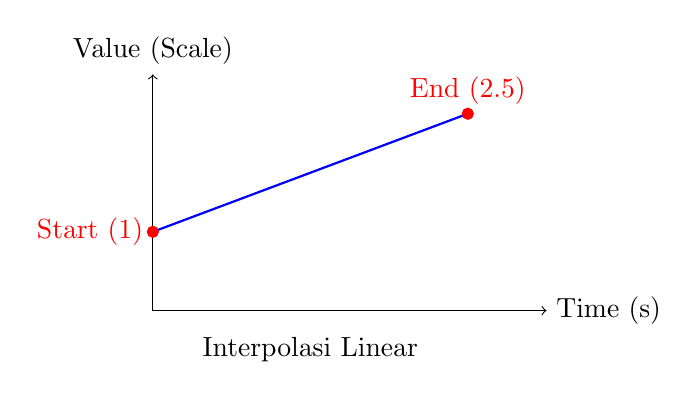
\begin{tikzpicture}
        \draw[->] (0,0) -- (5,0) node[right] {Time (s)};
        \draw[->] (0,0) -- (0,3) node[above] {Value (Scale)};
        
        \draw[blue, thick] (0,1) -- (4,2.5);
        \filldraw [red] (0,1) circle (2pt) node[anchor=east] {Start (1)};
        \filldraw [red] (4,2.5) circle (2pt) node[anchor=south] {End (2.5)};
        
        \node at (2, -0.5) {Interpolasi Linear};
    \end{tikzpicture}
    \caption{Visualisasi Kurva Animasi (Scale)}
    \label{fig:anim_curve}
\end{figure}

Sekarang jika Anda menekan Play di window Animation, lingkaran akan membesar lalu menghilang.
